\section{Experimental protocol}\label{sec:protocol}

The protocol was fixed in a written specification before any code was run, and its numerical settings were frozen after a one-seed pilot and before any final seed ran (\cref{sec:m-pilot}). Nothing was changed after the final runs started.

\subsection{Environments}

\paragraph{Finite mazes (\cref{def:env-finite}).}
A $7\times7$ lattice of cells $(x,y)$, in two layouts: \emph{open}, with \vn{env.cells.open}{49} free cells, and \emph{four rooms}, with walls at $x=3$ except $y\in\{1,5\}$ and at $y=3$ except $x\in\{1,5\}$, which leaves \vn{env.cells.4r}{40} free cells and four doorways.
The five actions move by one cell or stay; a move into a wall or out of the grid stays.
With probability $p_{\mathrm{slip}}=0.1$ the executed action is drawn uniformly from all five actions.
The start is the cell $(1,1)$ and the goals are $(5,1)$, $(5,5)$ and $(1,5)$; from the start, $(5,1)$ and $(1,5)$ are \vn{env.dist.side}{4} steps away and $(5,5)$ is \vn{env.dist.far}{8} steps away in both layouts, so the layouts differ by their walls, not by their shortest paths.
The transition matrix is used only by the oracle, the expert construction and the evaluation; its rank is \vn{env.rank.open}{49} or \vn{env.rank.4r}{40} (\cref{prop:env-finite}).

\paragraph{Continuous maze (\cref{def:env-cont}).}
The four-rooms layout rescaled to $[0,1]^2$: the free space is the open unit square minus the closed wall squares (area $\vn{env.cells.4r}{40}/\vn{env.cells.open}{49}$), the step length is one cell, $L=1/7$, and the start is the centre of cell $(1,1)$.
An action moves the agent by $L$ if the segment to the target is free, and otherwise stays; Gaussian noise of standard deviation $0.01$ is then added, redrawn until the noise segment is free.
This kernel has no clipping, no atom and no tunnelling, and a Lebesgue density bounded by about $\vn{const.p_max}{6366}$ (\cref{prop:env-cont}).

\paragraph{Evaluation reward and success.}
The reward of goal $g$ is $r_g(x)=\exp(-\lvert x-\bar g\rvert^2/(2w^2))$ with $\bar g$ the centre of the goal cell and $w=1/14$, read at the next state; in the finite maze $x$ is the cell centre.
Success (a ``hit'') means that some $s_t$ with $1\le t\le H$ lies in the goal region $\{\lvert x-\bar g\rvert\le1/14\}$, which in the finite maze is the goal cell.
Rewards and success are used for expert construction and evaluation only; no learner sees them.

\begin{figure}[ht]
\centering
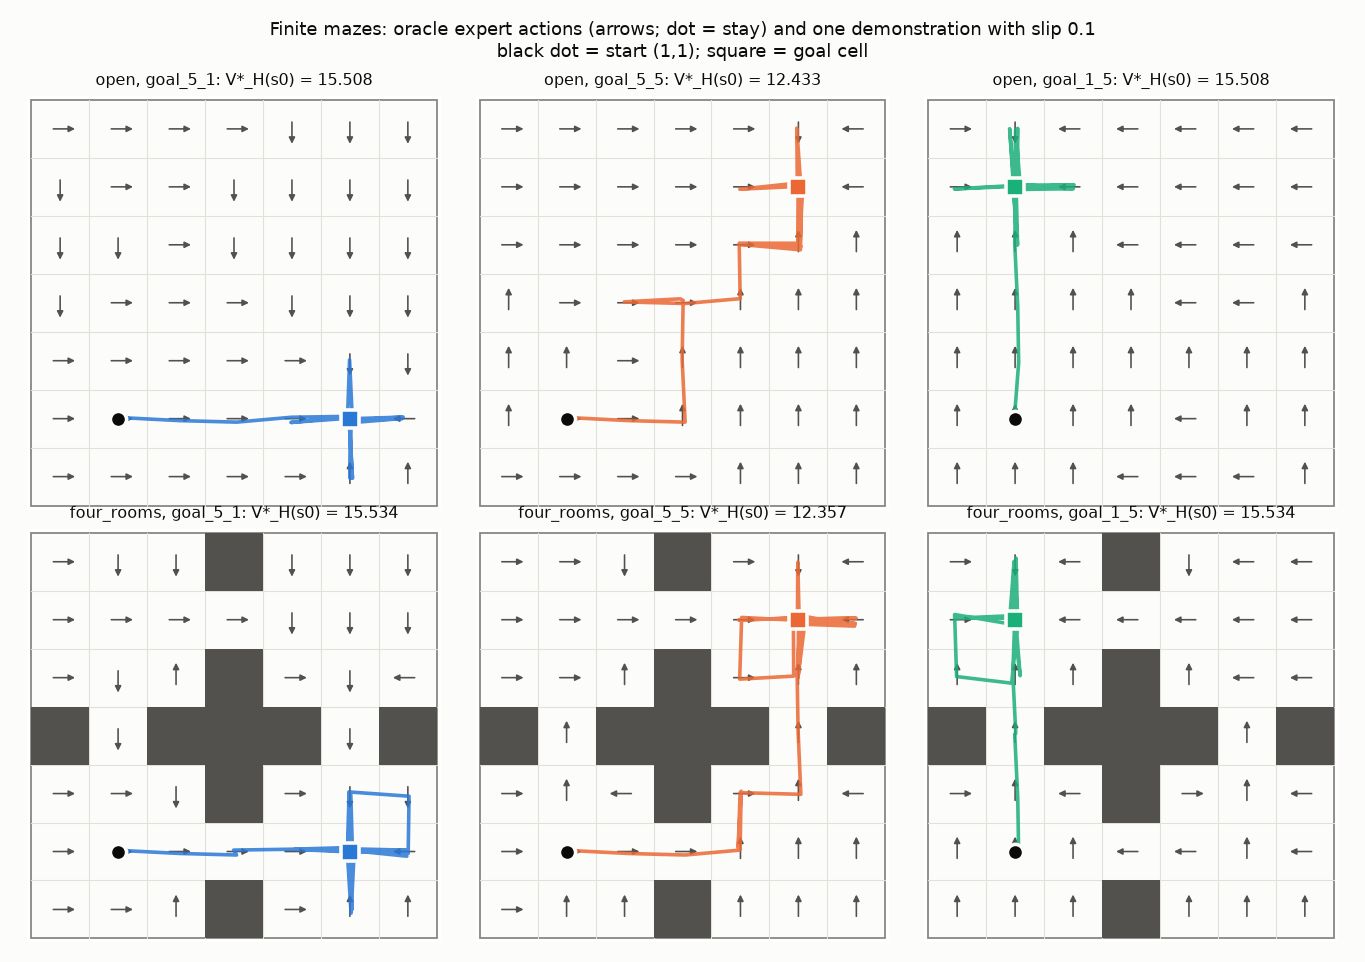
\includegraphics[width=0.86\textwidth]{figures/env_finite_expert_maps.png}
\caption{Finite mazes: actions of the certified oracle expert (arrows; a dot is ``stay'') and one demonstration with slip $0.1$, for the three goals of each layout. Illustration produced by \texttt{scripts/check\_environments.py} (laptop run, seed \vn{fig.env.seed}{20261005}, same environment configuration as the final runs); the final demonstrations are other draws from the same experts.}\label{fig:env-finite}
\end{figure}

\begin{figure}[ht]
\centering
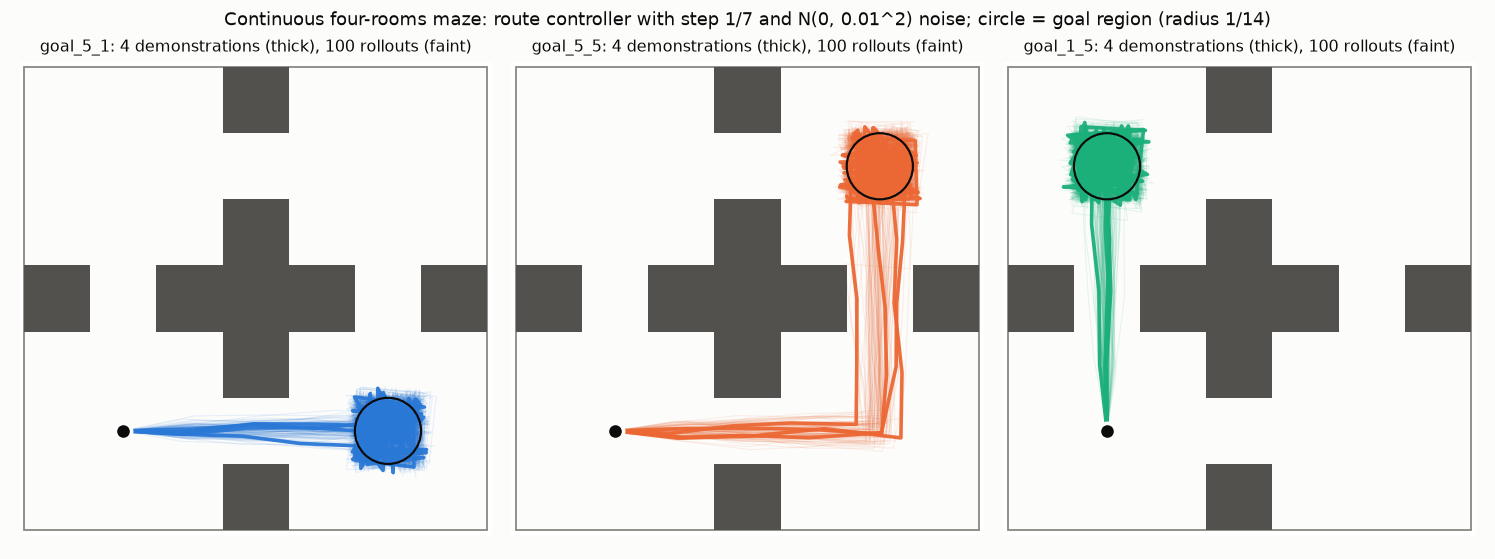
\includegraphics[width=\textwidth]{figures/env_continuous_expert_rollouts.png}
\caption{Continuous four-rooms maze: the route controller, with 4 demonstrations (thick) and 100 rollouts (faint) per goal; the circle is the goal region. Same source and caveat as \cref{fig:env-finite}.}\label{fig:env-cont}
\end{figure}

\subsection{Experts and data}

\paragraph{Experts.}
In the finite mazes the expert is the stationary optimal policy for $r_g$, computed by value iteration with a deterministic tie-breaking order and certified by its Bellman residual (\cref{prop:env-experts}(a)): over the six tasks the value-iteration residual is at most $\vn{s10.vi_res}{9.7\times10^{-13}}$ and the policy residual $\eta_{\pi^\star}$ at most $\vn{s10.pi_res}{1.1\times10^{-14}}$, and the expert's $H$-step return equals the $H$-step optimum $V^\star_H$ at the start state.
In the continuous maze the expert is a constructed route controller, $\pi_E(x)=\Gamma(\lfloor7x\rfloor)$ for a fixed table $\Gamma$ of shortest-path actions on free cells: a stationary state-feedback policy, as \DMFB{} requires, whose planned moves are almost surely never blocked (\cref{prop:env-experts}(b)--(c)). It is a reference controller, not a proven optimal policy. In the final evaluation it hits the goal in every rollout, and $\vn{s10.cont_expert_fig.lo}{72}$--$\vn{s10.cont_expert_fig.hi}{76}\%$ of its final states lie in the goal region.

\paragraph{Data.}
For every task and seed: $N_E=4$ demonstrations of $H=100$ transitions, of which learners receive the states only (actions are stored for the state--action diagnostic); for every layout and seed, a task-blind replay buffer for FB (\cref{sec:m-fb-loss}), whose coverage of every state--action pair was checked (at least \vn{s10.cover.finite}{137} visits per state--action pair in the finite buffers, and \vn{s10.cover.cont}{423} per pair of a free maze-lattice cell of side $1/7$ and an action in the continuous ones; at the finer resolution of the evaluation histogram the continuous coverage is incomplete near walls, \cref{sec:results-continuous}); and in the continuous maze, $2{,}000$ held-out expert trajectories as the evaluation reference.
All data were generated once, with recorded seeds and content hashes, and shared by all methods.

\subsection{Methods, settings and budgets}

\begin{table}[ht]
\centering\small
\caption{Frozen settings of the final runs (\texttt{configs/core.yaml}, \texttt{configs/compact\_ablations.yaml}).}\label{tab:settings}
\begin{tabularx}{\textwidth}{@{}>{\raggedright\arraybackslash}p{2.5cm}>{\raggedright\arraybackslash}X>{\raggedright\arraybackslash}X@{}}
\toprule
& finite mazes & continuous maze\\
\midrule
\multicolumn{3}{@{}l}{\textit{$f$-PG (Algorithm 1)}}\\
policy & tabular softmax logits & MLP, 2 $\tanh$ layers of 64, raw $(x,y)$\\
signal & smoothed counts, $\varepsilon=0.01$ & KDE, $h=0.05$, $\varepsilon=0.01$\\
updates & 25 Adam steps, lr $0.3$, 20 trajectories each & 50 Adam steps, lr $0.003$, 20 trajectories each\\
budget & $50{,}000$ learner transitions per task & $100{,}000$ learner transitions per task\\
\midrule
\multicolumn{3}{@{}l}{\textit{FB pretraining (Algorithm 2), one model per layout and seed, shared by its 3 goals}}\\
networks & $d=16$, width 64, one-hot inputs & $d=16$, width 64, raw $(x,y)$\\
data & $50{,}000$ replay transitions & $100{,}000$ replay transitions\\
updates & $10{,}000$ (batch $128+128$), Adam $3\times10^{-4}$ & $20{,}000$, same\\
policy & softmax, $\tau=1$, latents on the sphere $R=4$ & same\\
\midrule
\multicolumn{3}{@{}l}{\textit{\ERFB{} and \DMFB{} (Algorithm 3)}}\\
\DMFB & $K=60$, start times $0..40$, 300 Adam steps, lr $0.05$ & same\\
\bottomrule
\end{tabularx}
\end{table}

\paragraph{Suites and seeds.}
The \emph{core} suite has \vn{s10.core.jobs}{144} jobs: per seed, \vn{s10.perseed.fb}{3} FB pretraining runs, \vn{s10.perseed.adapt}{9} \ERFB/\DMFB{} adaptations, \vn{s10.perseed.fpg}{9} $f$-PG runs with $\JS$, their \vn{s10.perseed.eval}{18} evaluations and \vn{s10.perseed.evalexp}{9} expert evaluations. It covers both finite layouts and the continuous maze, three goals each, and the final seeds $0$, $1$ and $2$: \vn{s10.core.fpg}{27} $f$-PG runs, \vn{s10.core.fb}{9} FB models and \vn{s10.core.adapt}{27} adaptations.
The \emph{compact ablations} add \vn{s10.abl.new}{21} jobs on the four-rooms goal $(5,5)$: $f$-PG with $\KL(d\Vert q)$ and $\KL(q\Vert d)$ (\vn{s10.abl.fpg_new}{6} runs) and FB pretraining without the orthonormality penalty (\vn{s10.abl.fb_new}{3} models), with their adaptations and evaluations; the $\JS$ runs and the base FB models are the core's own jobs, reused by identifier.
Each job derives its random streams from its seed and labels, and evaluation streams are distinct from every training stream.
Some streams are shared on purpose, as common random numbers for paired comparisons: the $\KL$ runs share the initialization and the first batch of the $\JS$ run of the same seed; FB pretraining with and without the orthonormality penalty shares its initialization and minibatch streams; every checkpoint of a run, and every method of a goal and seed, is evaluated with the same evaluation random numbers, so continuous learning curves and paired differences carry correlated Monte Carlo noise (in the finite mazes the reported metrics are exact and only the Monte Carlo cross-checks use these streams); and the three seeds share one set of $2{,}000$ continuous reference rollouts (reference seed \vn{aJ.refseed}{314159}), so the standard deviations across seeds do not include the sampling variance of that reference.
The finite FB-imitation runs are \vn{s10.core.adapt.finite}{18} adaptations on \vn{s10.core.fb.finite}{6} pretrained FB models: the \ERFB{} and \DMFB{} runs of a goal and seed come from one adaptation job, and the three goals of a layout and seed share one model.
The budgets are the ceilings of the specification; they were not chosen as sufficient for convergence.

\subsection{Pilot and tuning scope}\label{sec:m-pilot}

A single-seed learning pilot (seed $\vn{pilot.seed}{999}$, distinct from the final seeds, four-rooms goal $(5,5)$ in both mazes) chose the settings that the specification left open, by rules declared before any final run: for $f$-PG the learning rate with the lowest last-checkpoint held-out divergence among three, and for FB the temperature with the best mean divergence and success over \ERFB{} and \DMFB{} in both mazes, together with the policy-entropy diagnostics. \Cref{tab:pilot} shows the evidence.

\begin{table}[ht]
\centering\small
\caption{Learning pilot (seed \vn{pilot.seed}{999}, four rooms, goal $(5,5)$): held-out divergence (nats) and success at the last checkpoint. Used only to choose the frozen settings; these are not results.}\label{tab:pilot}
% GENERATED by report/verify/make_tables.py from the saved run files (runs/jobs/*).
% Learning pilot (seed 999, four rooms, goal (5,5)): held-out metrics at the last checkpoint. Used only to freeze settings; not a result.
% Do not edit by hand: rerun  python3 report/verify/verify_results.py

\begin{tabular}{@{}llcccc@{}}
\toprule
setting & value & \multicolumn{2}{c}{finite: JS / success} & \multicolumn{2}{c}{continuous: JS / success}\\
\midrule
\fPG{} learning rate & 0.03 / 0.0003 & 0.361 & 0.708 & 0.508 & 0.602\\
\fPG{} learning rate & 0.1 / 0.001 & 0.160 & 1.000 & 0.486 & 0.776\\
\fPG{} learning rate & 0.3 / 0.003 (frozen) & 0.047 & 1.000 & 0.342 & 0.968\\
\fPG{} histogram signal & lr 0.001 & -- & -- & 0.488 & 0.700\\
\midrule
\ERFB, $\tau$ & 0.1 & 0.296 & 0.806 & 0.604 & 0.002\\
\DMFB, $\tau$ & 0.1 & 0.340 & 0.446 & 0.693 & 0.000\\
\ERFB, $\tau$ & 0.3 & 0.299 & 0.803 & 0.577 & 0.040\\
\DMFB, $\tau$ & 0.3 & 0.288 & 0.591 & 0.692 & 0.000\\
\ERFB, $\tau$ & 1 (frozen) & 0.179 & 0.983 & 0.581 & 0.128\\
\DMFB, $\tau$ & 1 (frozen) & 0.384 & 0.621 & 0.687 & 0.014\\
\bottomrule
\end{tabular}

\end{table}

The resulting settings have a narrow basis, which the results must be read with:
\begin{itemize}[nosep]
\item they were chosen on one goal of the four-rooms mazes with one seed; the open layout and the goals $(5,1)$ and $(1,5)$ inherit them untested;
\item both frozen $f$-PG learning rates are the largest of the tested grid, so a larger rate might have done better;
\item the $\KL$ ablations use the learning rate tuned for $\JS$;
\item in the pilot, \DMFB{} ended below its own \ERFB{} starting point at $\tau=1$: in the finite maze its held-out divergence rose from $\vn{s10.pilot.er_start}{0.179}$ at the \ERFB{} start to $\vn{s10.pilot.dm_end}{0.384}$ after the 300 latent steps, while its model objective fell from $\vn{s10.pilot.l0}{-1456}$ to $\vn{s10.pilot.l1}{-1647}$;
\item in the pilot the continuous FB Gram matrix was nearly singular ($\lambda_{\min}(\hat G_B)\approx\vn{s10.pilot.lmin}{2\times10^{-5}}$), and continuous \ERFB{} and \DMFB{} failed.
\end{itemize}
The \DMFB{} settings, the network sizes and the budgets were not in the pilot grid and were kept at their initial values.

\subsection{Evaluation and operational thresholds}

\paragraph{Finite mazes: exact evaluation.}
For every checkpointed policy the oracle computes, from $P$: the occupancy divergence $\JS(d^+_{\pi,H},q_E)$ against the exact expert occupancy, the state--action diagnostic $\JS(d^{\SA}_{\pi,H},q^{\SA}_E)$, the exact $H$-step return and its gap to $V^\star_H$, and the exact hit probability; 200 Monte Carlo rollouts cross-check them. For FB models it also computes the exact model error of \cref{thm:m-fb-approx}.

\paragraph{Continuous maze: Monte Carlo evaluation.}
500 fresh rollouts per checkpoint give the success rate, the return, the fraction of final states in the goal region and the occupancy divergence: a plug-in $\JS$ between the masses that the policy's rollouts and the $2{,}000$ reference rollouts put on the \vn{env.hist_cells}{356} free-space histogram cells, with the discount weights $\gamma^t/(nZ_H)$. This plug-in estimate is biased upward; the expert's own row measures its floor, $\vn{s10.floor.lo}{0.0005}$ to $\vn{s10.floor.hi}{0.0013}$ nats.

\paragraph{Checkpoints and thresholds.}
$f$-PG policies are evaluated every 5 iterations, \ERFB{} and the final \DMFB{} latent at every FB snapshot, and the \DMFB{} iterates every 50 steps at the final snapshot. All tables use the \emph{last} checkpoint, i.e.\ the full budget.
A run \emph{meets the operational thresholds} at a checkpoint if $\JS\le0.10$ nats and success $\ge0.80$. These thresholds were declared in the specification and kept unchanged; they are study choices, not universal standards. ``First reached'' is the first assessed checkpoint at which both hold, in learner transitions for $f$-PG and in FB pretraining updates for \ERFB{} and \DMFB{}, where \DMFB{} is assessed after its completed 300 latent steps at each snapshot; ``not reached'' means at no assessed checkpoint within the budget.
With $f$-PG evaluated every $\vn{fpg.interval.f}{10{,}000}$ learner transitions, a first hit is an observed bound at that resolution, not a measured sample requirement.

\subsection{Execution and provenance}

All runs executed sequentially on the CPU of the author's laptop (\vn{s10.threads}{4} PyTorch threads, NumPy and BLAS thread counts neither set nor recorded; Windows, Python \vn{s10.python}{3.11.16}, PyTorch \vn{s10.torch}{2.14.1}), chosen because the pilot measured it faster than the laptop GPU for these small networks.
The core suite ran on \vn{time.core.date}{5 October 2026} from \vn{time.core.start}{21:46:55} to \vn{time.core.end}{22:02:35} UTC, the ablations from \vn{time.abl.start}{22:20:00} to \vn{time.abl.end}{22:22:55} UTC; all \vn{s10.jobs_first_attempt}{165} jobs completed at their first attempt, with no failure or interruption, and the peak process memory was $\vn{s10.peak_rss}{823}$~MiB.
Every job records its configuration, code, data and dependency hashes, device, wall times and outputs; the provenance audit of the results (\texttt{scripts/audit\_results.py}) reports no error and no warning, and a second implementation (\texttt{report/verify/verify\_results.py}), which recomputes the results from the raw run files without the project's analysis code, reproduces every table (\cref{app:repro}).
